\documentclass{article}

\usepackage{arxiv}

\usepackage[utf8]{inputenc} % allow utf-8 input
\usepackage[T1]{fontenc}    % use 8-bit T1 fonts
\usepackage{lmodern}        % https://github.com/rstudio/rticles/issues/343
\usepackage{hyperref}       % hyperlinks
\usepackage{url}            % simple URL typesetting
\usepackage{booktabs}       % professional-quality tables
\usepackage{amsfonts}       % blackboard math symbols
\usepackage{nicefrac}       % compact symbols for 1/2, etc.
\usepackage{microtype}      % microtypography
\usepackage{graphicx}

\title{gibbonNetR: an R Package for the Use of Convolutional Neural
Networks and Transfer Learning on Acoustic Data}

\author{
    Dena Jane Clink
   \\
    K. Lisa Yang Center for Conservation Bioacoustics \\
    Cornell Lab of Ornithology, Cornell University, Ithaca, New York,
United States \\
   \\
  \texttt{\href{mailto:dena.clink@cornell.edu}{\nolinkurl{dena.clink@cornell.edu}}} \\
   \And
    Abdul Hamid Ahmad
   \\
    Institute for Tropical Biology and Conservation \\
    Universiti Malaysia Sabah (UMS), Kota Kinabalu, Sabah, Malaysia \\
   \\
  \texttt{} \\
  }

% Pandoc syntax highlighting
\usepackage{color}
\usepackage{fancyvrb}
\newcommand{\VerbBar}{|}
\newcommand{\VERB}{\Verb[commandchars=\\\{\}]}
\DefineVerbatimEnvironment{Highlighting}{Verbatim}{commandchars=\\\{\}}
% Add ',fontsize=\small' for more characters per line
\usepackage{framed}
\definecolor{shadecolor}{RGB}{248,248,248}
\newenvironment{Shaded}{\begin{snugshade}}{\end{snugshade}}
\newcommand{\AlertTok}[1]{\textcolor[rgb]{0.94,0.16,0.16}{#1}}
\newcommand{\AnnotationTok}[1]{\textcolor[rgb]{0.56,0.35,0.01}{\textbf{\textit{#1}}}}
\newcommand{\AttributeTok}[1]{\textcolor[rgb]{0.13,0.29,0.53}{#1}}
\newcommand{\BaseNTok}[1]{\textcolor[rgb]{0.00,0.00,0.81}{#1}}
\newcommand{\BuiltInTok}[1]{#1}
\newcommand{\CharTok}[1]{\textcolor[rgb]{0.31,0.60,0.02}{#1}}
\newcommand{\CommentTok}[1]{\textcolor[rgb]{0.56,0.35,0.01}{\textit{#1}}}
\newcommand{\CommentVarTok}[1]{\textcolor[rgb]{0.56,0.35,0.01}{\textbf{\textit{#1}}}}
\newcommand{\ConstantTok}[1]{\textcolor[rgb]{0.56,0.35,0.01}{#1}}
\newcommand{\ControlFlowTok}[1]{\textcolor[rgb]{0.13,0.29,0.53}{\textbf{#1}}}
\newcommand{\DataTypeTok}[1]{\textcolor[rgb]{0.13,0.29,0.53}{#1}}
\newcommand{\DecValTok}[1]{\textcolor[rgb]{0.00,0.00,0.81}{#1}}
\newcommand{\DocumentationTok}[1]{\textcolor[rgb]{0.56,0.35,0.01}{\textbf{\textit{#1}}}}
\newcommand{\ErrorTok}[1]{\textcolor[rgb]{0.64,0.00,0.00}{\textbf{#1}}}
\newcommand{\ExtensionTok}[1]{#1}
\newcommand{\FloatTok}[1]{\textcolor[rgb]{0.00,0.00,0.81}{#1}}
\newcommand{\FunctionTok}[1]{\textcolor[rgb]{0.13,0.29,0.53}{\textbf{#1}}}
\newcommand{\ImportTok}[1]{#1}
\newcommand{\InformationTok}[1]{\textcolor[rgb]{0.56,0.35,0.01}{\textbf{\textit{#1}}}}
\newcommand{\KeywordTok}[1]{\textcolor[rgb]{0.13,0.29,0.53}{\textbf{#1}}}
\newcommand{\NormalTok}[1]{#1}
\newcommand{\OperatorTok}[1]{\textcolor[rgb]{0.81,0.36,0.00}{\textbf{#1}}}
\newcommand{\OtherTok}[1]{\textcolor[rgb]{0.56,0.35,0.01}{#1}}
\newcommand{\PreprocessorTok}[1]{\textcolor[rgb]{0.56,0.35,0.01}{\textit{#1}}}
\newcommand{\RegionMarkerTok}[1]{#1}
\newcommand{\SpecialCharTok}[1]{\textcolor[rgb]{0.81,0.36,0.00}{\textbf{#1}}}
\newcommand{\SpecialStringTok}[1]{\textcolor[rgb]{0.31,0.60,0.02}{#1}}
\newcommand{\StringTok}[1]{\textcolor[rgb]{0.31,0.60,0.02}{#1}}
\newcommand{\VariableTok}[1]{\textcolor[rgb]{0.00,0.00,0.00}{#1}}
\newcommand{\VerbatimStringTok}[1]{\textcolor[rgb]{0.31,0.60,0.02}{#1}}
\newcommand{\WarningTok}[1]{\textcolor[rgb]{0.56,0.35,0.01}{\textbf{\textit{#1}}}}

% tightlist command for lists without linebreak
\providecommand{\tightlist}{%
  \setlength{\itemsep}{0pt}\setlength{\parskip}{0pt}}


% Pandoc citation processing
\newlength{\cslhangindent}
\setlength{\cslhangindent}{1.5em}
\newlength{\csllabelwidth}
\setlength{\csllabelwidth}{3em}
\newlength{\cslentryspacingunit} % times entry-spacing
\setlength{\cslentryspacingunit}{\parskip}
% for Pandoc 2.8 to 2.10.1
\newenvironment{cslreferences}%
  {}%
  {\par}
% For Pandoc 2.11+
\newenvironment{CSLReferences}[2] % #1 hanging-ident, #2 entry spacing
 {% don't indent paragraphs
  \setlength{\parindent}{0pt}
  % turn on hanging indent if param 1 is 1
  \ifodd #1
  \let\oldpar\par
  \def\par{\hangindent=\cslhangindent\oldpar}
  \fi
  % set entry spacing
  \setlength{\parskip}{#2\cslentryspacingunit}
 }%
 {}
\usepackage{calc}
\newcommand{\CSLBlock}[1]{#1\hfill\break}
\newcommand{\CSLLeftMargin}[1]{\parbox[t]{\csllabelwidth}{#1}}
\newcommand{\CSLRightInline}[1]{\parbox[t]{\linewidth - \csllabelwidth}{#1}\break}
\newcommand{\CSLIndent}[1]{\hspace{\cslhangindent}#1}

\usepackage[left]{lineno}
\linenumbers
\usepackage{float}
\begin{document}
\maketitle


\begin{abstract}
Automated detection of acoustic signals is crucial for effective
monitoring of vocal animals and their habitats across large spatial and
temporal scales. Recent advances in deep learning have made high
performing automated detection approaches more accessible two more
practitioners. However, there are few deep learning approaches that can
be implemented natively in R. The `torch for R' ecosystem has made the
use of transfer learning with convolutional neural networks accessible
for R users. Here we provide an R package and workflow to use transfer
learning for the automated detection of acoustics signals from passive
acoustic monitoring (PAM) data collected in Sabah, Malaysia. The package
provides functions to create spectogram images from PAM data, compare
the performance of different pre-trained CNN architectures, and deploy
trained models over directories of sound files.
\end{abstract}

\keywords{
    deep learning
   \and
    passive acoustic monitoring
   \and
    gibbon
   \and
    automated detection
  }

\hypertarget{introduction}{%
\section{Introduction}\label{introduction}}

\hypertarget{passive-acoustic-monitoring}{%
\subsection{\texorpdfstring{\emph{Passive acoustic
monitoring}}{Passive acoustic monitoring}}\label{passive-acoustic-monitoring}}

We are in a biodiversity crisis, and there is a great need for the
ability to rapidly assess biodiversity in order to understand and
mitigate anthropogenic impacts. One approach that can be especially
effective for monitoring of vocal yet cryptic animals is the use of
passive acoustic monitoring (Gibb et al. 2018), a technique that relies
autonomous acoustic recording units. PAM allows researchers to monitor
vocal animals and their habitats, at temporal and spatial scales that
are impossible to achieve using only human observers. Interest in use of
PAM in terrestrial environments has increased substantially in recent
years (Sugai et al. 2019), due to reduced price of the recording units
and improved battery life and data storage capabilities. However, the
use of PAM often leads to the collection of terabytes of data that is
time- and cost-prohibitive to analyze manually.

\hypertarget{automated-detection}{%
\subsection{\texorpdfstring{\emph{Automated
detection}}{Automated detection}}\label{automated-detection}}

Some commonly used non-deep learning approaches for the automated
detection of acoustic signals in terrestrial PAM data include binary
point matching (Katz, Hafner, and Donovan 2016), spectrogram
cross-correlation (Balantic and Donovan 2020), or the use of a band-
limited energy detector and subsequent classifier, such as support
vector machine (Clink et al. 2023; Kalan et al. 2015). Recent advances
in deep learning have revolutionized image and speech recognition
(LeCun, Bengio, and Hinton 2015 ), with important cross-over for the
analysis of PAM data. Traditional approaches to machine learning relied
heavily on feature engineering, as early machine learning algorithms
required a reduced set of representative features, such as features
estimated from the spectrogram. Deep learning does not require feature
engineering (Stevens, Antiga, and Viehmann 2020) . Convolutional neural
networks (CNNs) --- one of the most effective deep learning
algorithms---are useful for processing data that have a `grid-like
topology', such as image data that can be considered a 2-dimensional
grid of pixels (Goodfellow, Bengio, and Courville 2016). The
`convolutional' layer learns the feature representations of the inputs;
these convolutional layers consist of a set of filters which are
basically two-dimensional matrices of numbers and the primary parameter
is the number of filters (Gu et al. 2018). Therefore, with CNN's there
is no feature engineering required. However, if training data are
scarce, overfitting may occur as representations of images tend to be
large with many variables (LeCun, Bengio, and others 1995).

Transfer learning is an approach wherein the architecture of a
pretrained CNN (which is generally trained on a large dataset) is
applied to a new classification problem. For example, CNNs trained on
the ImageNet dataset of \textgreater{} 1 million images (Deng et al.
2009)such as ResNet have been applied to automated
detection/classification of primate and bird species from PAM data
(Dufourq et al. 2022; Ruan et al. 2022). At the most basic level,
transfer learning in computer vision applications retains the feature
extraction or embedding layers, and modifies the last few classification
layers to be trained for a new classification task (Dufourq et al.
2022). Transfer learning has been shown to outperform CNNs trained with
random initial weights (Tan et al. 2018). Transfer learning is
particularly appropriate when there is a paucity of training data
(Weiss, Khoshgoftaar, and Wang 2016), such as common in PAM data.

\hypertarget{torch-for-r-ecosystem}{%
\subsection{\texorpdfstring{\emph{`torch for R'
ecosystem}}{`torch for R' ecosystem}}\label{torch-for-r-ecosystem}}

The two most popular open-source programming languages are R and Python
(Scavetta and Angelov 2021). Python has surpassed R in terms of overall
popularity, but R remains an important language for the life sciences
(Lawlor et al. 2022). `Keras' (Chollet and others 2015), `PyTorch'
(Paszke et al. 2019) and `Tensorflow' (Martín Abadi et al. 2015) are
some of the more popular neural network libraries; these libraries were
all initially developed for the Python programming language. Until
recently, deep learning implementations in R relied on the `reticulate'
package which served as an interface to Python (Ushey, Allaire, and Tang
2022). However, the recent release of the `torch for R' ecosystem
provides a framework based on `PyTorch' that runs natively in R and has
no dependency on Python (Falbel 2023). Running natively in R means more
straightforward installation, and higher accessibility for users of the
R programming environment. Keydana (2023) provides tutorials for
transfer learning in the `torch for R' ecosystem, and the functions in
`gibbonNetR' rely heavily on these tutorials.

\hypertarget{overview}{%
\section{Overview}\label{overview}}

This package provides functions

\hypertarget{usage}{%
\section{Usage}\label{usage}}

\hypertarget{first-we-create-spectrogram-images}{%
\subsection{First we create spectrogram
images}\label{first-we-create-spectrogram-images}}

\begin{figure}[H]

{\centering 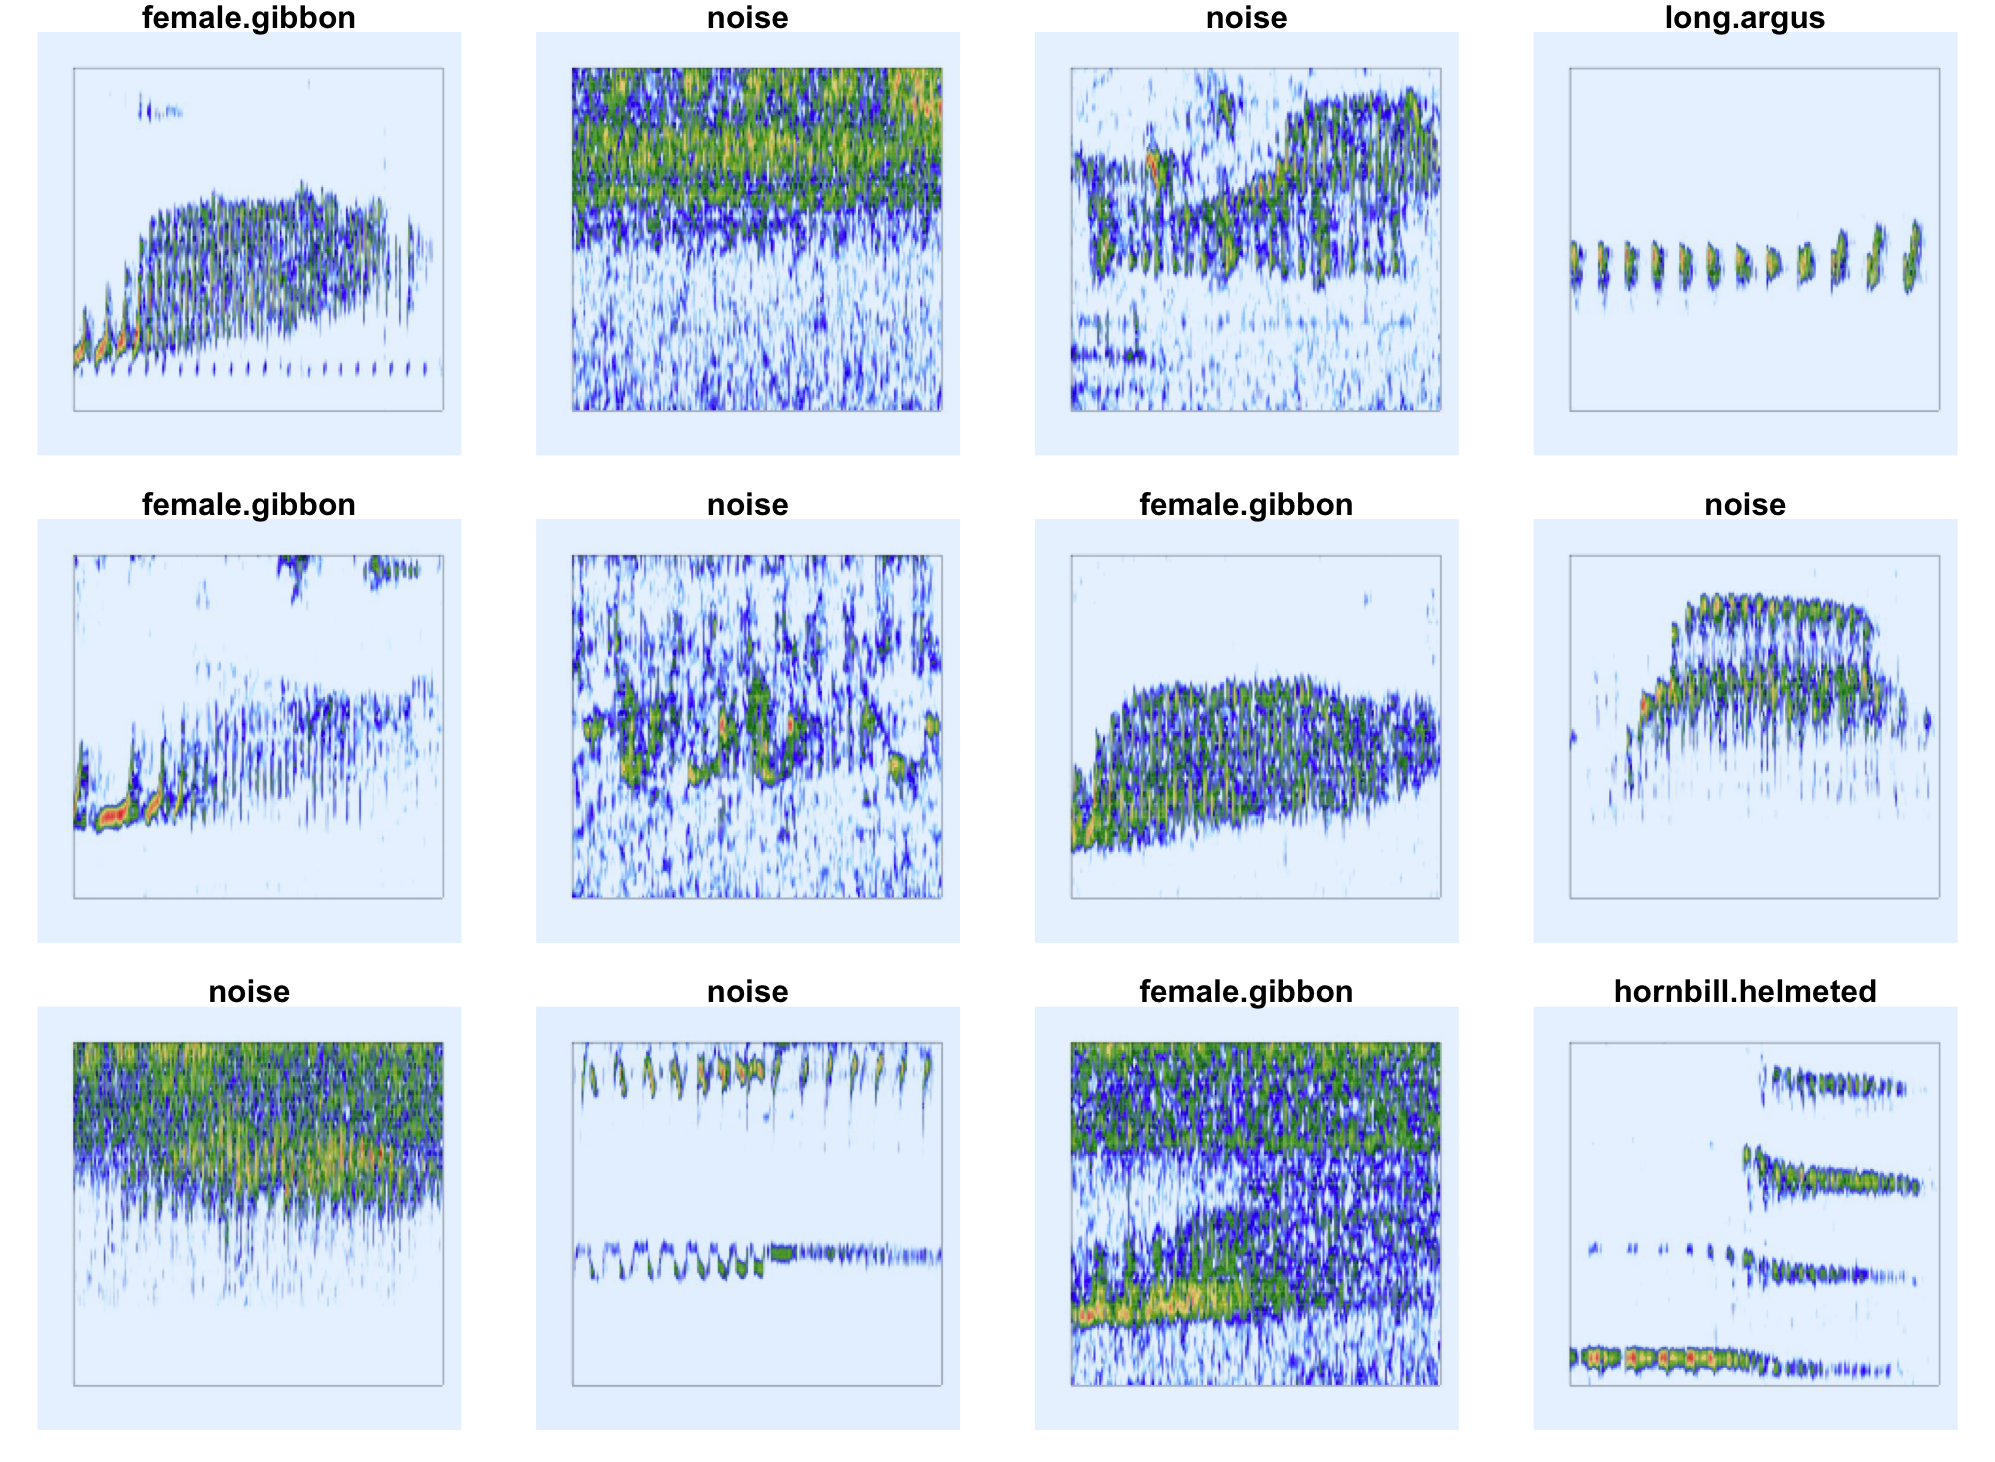
\includegraphics[width=0.75\linewidth]{../../README_files/spectro} 

}

\caption{Spectrograms of training clips for CNNs}\label{fig:unnamed-chunk-1}
\end{figure}

\hypertarget{then-we-train-the-model}{%
\subsection{Then we train the model}\label{then-we-train-the-model}}

\begin{Shaded}
\begin{Highlighting}[]
\NormalTok{gibbonNetR}\SpecialCharTok{::}\FunctionTok{train\_alexNet}\NormalTok{(}\AttributeTok{input.data.path=}\NormalTok{input.data.path,}
                          \AttributeTok{test.data=}\NormalTok{test.data.path,}
                          \AttributeTok{unfreeze =}\NormalTok{ unfreeze.param,}
                          \AttributeTok{epoch.iterations=}\NormalTok{epoch.iterations,}
                          \AttributeTok{early.stop =} \StringTok{"yes"}\NormalTok{,}
                          \AttributeTok{output.base.path =} \StringTok{"data/"}\NormalTok{,}
                          \AttributeTok{trainingfolder=}\NormalTok{trainingfolder.short,}
                          \AttributeTok{positive.class=}\StringTok{"Gibbons"}\NormalTok{,}
                          \AttributeTok{negative.class=}\StringTok{"Noise"}\NormalTok{)}
\end{Highlighting}
\end{Shaded}

\hypertarget{we-can-compare-the-performance-of-different-cnn-architectures}{%
\subsection{We can compare the performance of different CNN
architectures}\label{we-can-compare-the-performance-of-different-cnn-architectures}}

\begin{figure}[H]

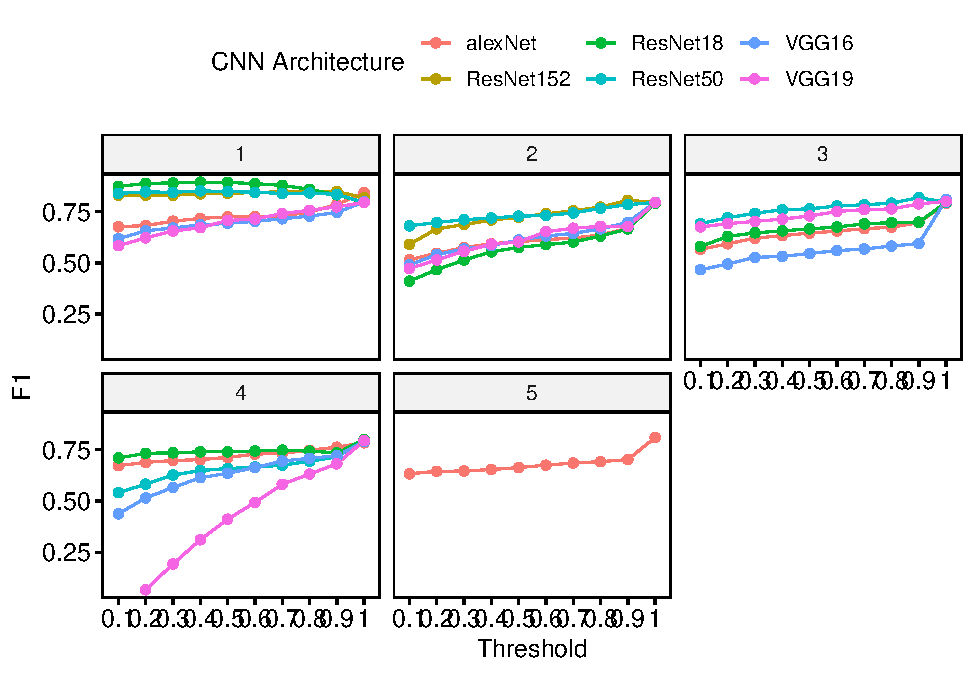
\includegraphics{gibbonNetRMSarxiv_files/figure-latex/unnamed-chunk-3-1} \hfill{}

\caption{Evaluating performance of pretrained CNNs}\label{fig:unnamed-chunk-3}
\end{figure}

\hypertarget{discussion}{%
\section{Discussion}\label{discussion}}

\hypertarget{acknowledgments}{%
\section{Acknowledgments}\label{acknowledgments}}

So long and thanks for all the fish.

\hypertarget{references}{%
\section*{References}\label{references}}
\addcontentsline{toc}{section}{References}

\hypertarget{refs}{}
\begin{CSLReferences}{1}{0}
\leavevmode\vadjust pre{\hypertarget{ref-balantic2020}{}}%
Balantic, Cathleen, and Therese Donovan. 2020. {``AMMonitor: Remote
Monitoring of Biodiversity in an Adaptive Framework with r.''}
\emph{Methods in Ecology and Evolution} 11 (7): 869877.

\leavevmode\vadjust pre{\hypertarget{ref-chollet2015}{}}%
Chollet, François, and others. 2015. {``Keras.''}
\url{https://keras.io}.

\leavevmode\vadjust pre{\hypertarget{ref-clink2023}{}}%
Clink, Dena J., Isabel Kier, Abdul Hamid Ahmad, and Holger Klinck. 2023.
{``A Workflow for the Automated Detection and Classification of Female
Gibbon Calls from Long-Term Acoustic Recordings.''} \emph{Frontiers in
Ecology and Evolution} 11.
\url{https://www.frontiersin.org/articles/10.3389/fevo.2023.1071640}.

\leavevmode\vadjust pre{\hypertarget{ref-deng2009}{}}%
Deng, Jia, Wei Dong, Richard Socher, Li-Jia Li, Kai Li, and Li Fei-Fei.
2009. {``Imagenet: A Large-Scale Hierarchical Image Database.''} In,
248255. Ieee.

\leavevmode\vadjust pre{\hypertarget{ref-dufourq2022}{}}%
Dufourq, Emmanuel, Carly Batist, Ruben Foquet, and Ian Durbach. 2022.
{``Passive Acoustic Monitoring of Animal Populations with Transfer
Learning.''} \emph{Ecological Informatics} 70: 101688.
https://doi.org/\url{https://doi.org/10.1016/j.ecoinf.2022.101688}.

\leavevmode\vadjust pre{\hypertarget{ref-falbel2023}{}}%
Falbel, Daniel. 2023. \emph{Luz: Higher Level 'API' for 'Torch'}.
\url{https://CRAN.R-project.org/package=luz}.

\leavevmode\vadjust pre{\hypertarget{ref-gibb2018}{}}%
Gibb, Rory, Ella Browning, Paul Glover-Kapfer, and Kate E. Jones. 2018.
{``Emerging Opportunities and Challenges for Passive Acoustics in
Ecological Assessment and Monitoring.''} \emph{Methods in Ecology and
Evolution}, October. \url{https://doi.org/10.1111/2041-210X.13101}.

\leavevmode\vadjust pre{\hypertarget{ref-goodfellow2016}{}}%
Goodfellow, Ian, Yoshua Bengio, and Aaron Courville. 2016. \emph{Deep
Learning}. MIT Press.

\leavevmode\vadjust pre{\hypertarget{ref-gu2018}{}}%
Gu, Jiuxiang, Zhenhua Wang, Jason Kuen, Lianyang Ma, Amir Shahroudy,
Bing Shuai, Ting Liu, et al. 2018. {``Recent Advances in Convolutional
Neural Networks.''} \emph{Pattern Recognition} 77: 354377.

\leavevmode\vadjust pre{\hypertarget{ref-kalan2015}{}}%
Kalan, Ammie K., Roger Mundry, Oliver J J Wagner, Stefanie Heinicke,
Christophe Boesch, and Hjalmar S. Kühl. 2015. {``Towards the Automated
Detection and Occupancy Estimation of Primates Using Passive Acoustic
Monitoring.''} \emph{Ecological Indicators} 54 (July 2015): 217226.
\url{https://doi.org/10.1016/j.ecolind.2015.02.023}.

\leavevmode\vadjust pre{\hypertarget{ref-katz2016}{}}%
Katz, Jonathan, Sasha D Hafner, and Therese Donovan. 2016. {``Assessment
of Error Rates in Acoustic Monitoring with the r Package monitoR.''}
\emph{Bioacoustics} 25 (2): 177196.

\leavevmode\vadjust pre{\hypertarget{ref-keydana2023}{}}%
Keydana, Sigrid. 2023. \emph{Deep Learning and Scientific Computing with
r Torch}. CRC Press.

\leavevmode\vadjust pre{\hypertarget{ref-lawlor2022}{}}%
Lawlor, Jake, Francis Banville, Norma-Rocio Forero-Muñoz, Katherine
Hébert, Juan Andrés Martínez-Lanfranco, Pierre Rogy, and A. Andrew M.
MacDonald. 2022. {``Ten Simple Rules for Teaching Yourself R.''}
\emph{PLOS Computational Biology} 18 (9): e1010372.
\url{https://doi.org/10.1371/journal.pcbi.1010372}.

\leavevmode\vadjust pre{\hypertarget{ref-lecun2015}{}}%
LeCun, Yann, Yoshua Bengio, and Geoffrey Hinton. 2015. {``Deep
Learning.''} \emph{Nature} 521 (7553): 436--44.
\url{https://doi.org/10.1038/nature14539}.

\leavevmode\vadjust pre{\hypertarget{ref-lecun1995}{}}%
LeCun, Yann, Yoshua Bengio, and others. 1995. {``Convolutional Networks
for Images, Speech, and Time Series.''} \emph{The Handbook of Brain
Theory and Neural Networks} 3361 (10): 1995.

\leavevmode\vadjust pre{\hypertarget{ref-martuxednabadi2015}{}}%
Martín Abadi, Ashish Agarwal, Paul Barham, Eugene Brevdo, Zhifeng Chen,
Craig Citro, Greg S. Corrado, et al. 2015. {``TensorFlow: Large-Scale
Machine Learning on Heterogeneous Systems.''}
\url{https://www.tensorflow.org/}.

\leavevmode\vadjust pre{\hypertarget{ref-paszke2019}{}}%
Paszke, Adam, Sam Gross, Francisco Massa, Adam Lerer, James Bradbury,
Gregory Chanan, Trevor Killeen, et al. 2019. {``PyTorch: An Imperative
Style, High-Performance Deep Learning Library.''} In, 80248035. Curran
Associates, Inc.
\url{http://papers.neurips.cc/paper/9015-pytorch-an-imperative-style-high-performance-deep-learning-library.pdf}.

\leavevmode\vadjust pre{\hypertarget{ref-ruan2022}{}}%
Ruan, Wenda, Keyi Wu, Qingchun Chen, and Chengyun Zhang. 2022.
{``ResNet-Based Bio-Acoustics Presence Detection Technology of Hainan
Gibbon Calls.''} \emph{Applied Acoustics} 198: 108939.
https://doi.org/\url{https://doi.org/10.1016/j.apacoust.2022.108939}.

\leavevmode\vadjust pre{\hypertarget{ref-scavetta2021}{}}%
Scavetta, Rick J, and Boyan Angelov. 2021. \emph{Python and r for the
Modern Data Scientist}. O'Reilly Media, Inc.

\leavevmode\vadjust pre{\hypertarget{ref-stevens2020}{}}%
Stevens, Eli, Luca Antiga, and Thomas Viehmann. 2020. \emph{Deep
Learning with PyTorch}. Simon; Schuster.

\leavevmode\vadjust pre{\hypertarget{ref-sugai2019}{}}%
Sugai, Larissa Sayuri Moreira, Thiago Sanna Freire Silva, José Wagner
Ribeiro, and Diego Llusia. 2019. {``Terrestrial Passive Acoustic
Monitoring: Review and Perspectives.''} \emph{BioScience} 69 (1): 1525.
\url{https://doi.org/10.1093/biosci/biy147}.

\leavevmode\vadjust pre{\hypertarget{ref-tan2018}{}}%
Tan, Chuanqi, Fuchun Sun, Tao Kong, Wenchang Zhang, Chao Yang, and
Chunfang Liu. 2018. {``A Survey on Deep Transfer Learning.''} In,
270279. Springer.

\leavevmode\vadjust pre{\hypertarget{ref-ushey2022}{}}%
Ushey, Kevin, J. J. Allaire, and Yuan Tang. 2022. \emph{Reticulate:
Interface to 'Python'}.

\leavevmode\vadjust pre{\hypertarget{ref-weiss2016}{}}%
Weiss, Karl, Taghi M Khoshgoftaar, and DingDing Wang. 2016. {``A Survey
of Transfer Learning.''} \emph{Journal of Big Data} 3 (1): 140.

\end{CSLReferences}

\bibliographystyle{unsrt}
\bibliography{references.bib}


\end{document}
